% !TEX TS-program = pdflatex
% !TEX encoding = UTF-8 Unicode

% This is a simple template for a LaTeX document using the "article" class.
% See "book", "report", "letter" for other types of document.

\documentclass[11pt, preview]{standalone} % use larger type; default would be 10pt

\usepackage[utf8]{inputenc} % set input encoding (not needed with XeLaTeX)


\usepackage{../../markup}
%%% Examples of Article customizations
% These packages are optional, depending whether you want the features they provide.
% See the LaTeX Companion or other references for full information.

%%% PAGE DIMENSIONS
\usepackage{geometry} % to change the page dimensions
\geometry{a4paper} % or letterpaper (US) or a5paper or....
% \geometry{margin=2in} % for example, change the margins to 2 inches all round
% \geometry{landscape} % set up the page for landscape
%   read geometry.pdf for detailed page layout information

\usepackage{graphicx} % support the \includegraphics command and options
\usepackage{color, tikz}
% \usepackage[parfill]{parskip} % Activate to begin paragraphs with an empty line rather than an indent

%%% PACKAGES
\usepackage{amsmath, amsfonts,amssymb}
\usepackage{booktabs} % for much better looking tables
\usepackage{array} % for better arrays (eg matrices) in maths
\usepackage{paralist} % very flexible & customisable lists (eg. enumerate/itemize, etc.)
\usepackage{verbatim} % adds environment for commenting out blocks of text & for better verbatim
\usepackage{subfig} % make it possible to include more than one captioned figure/table in a single float
% These packages are all incorporated in the memoir class to one degree or another...

%%% HEADERS & FOOTERS
\usepackage{fancyhdr} % This should be set AFTER setting up the page geometry
\pagestyle{fancy} % options: empty , plain , fancy
\renewcommand{\headrulewidth}{0pt} % customise the layout...
\lhead{}\chead{}\rhead{}
\lfoot{}\cfoot{\thepage}\rfoot{}

%%% SECTION TITLE APPEARANCE
\usepackage{sectsty}
\allsectionsfont{\sffamily\mdseries\upshape} % (See the fntguide.pdf for font help)
% (This matches ConTeXt defaults)

%%% ToC (table of contents) APPEARANCE
\usepackage[nottoc,notlof,notlot]{tocbibind} % Put the bibliography in the ToC
\usepackage[titles,subfigure]{tocloft} % Alter the style of the Table of Contents
\renewcommand{\cftsecfont}{\rmfamily\mdseries\upshape}
\renewcommand{\cftsecpagefont}{\rmfamily\mdseries\upshape} % No bold!

\newcommand{\N}{\mathbb{N}}
\newcommand{\Prob}{\mathbb{P}}
\newcommand{\Z}{\mathbb{Z}}
\newcommand{\R}{\mathbb{R}}
\newcommand{\Q}{\mathbb{Q}}
%%% END Article customizations

%%% The "real" document content comes below...

\date{} % Activate to display a given date or no date (if empty),
         % otherwise the current date is printed 

\begin{document}
\config{name}{Independence, Hashing and Bin Packing}
\noindent{\bf Independence, Hashing and Bin Packing}.

\begin{enumerate}
\item {\bf Independence.} For each of the following examples, decide whether the listed events are mutually independent, pairwise independent, or neither (if the events are mutually independent, there is no need to also select pairwise independent).
\begin{enumerate}
\item The event of drawing a jack of hearts from the deck and the event of drawing a jack of clubs from the same deck. 
\begin{Multi}
Recall the definition of independence--is the probability of both events equal to the product of the probabilities of each event? Should one event influence the probability of the other?
\begin{itemize}
\FalseChoice\item Mutually Independent
\FalseChoice\item Only Pairwise Independent
\TrueChoice\item Neither
\end{itemize}
\end{Multi}
%-----------------------------------
\item The event of drawing a jack of hearts from the deck and the event of drawing an ace of diamonds from the same deck. 
\begin{Multi}
Recall the definition independence--is the probability of both events equal to the product of the probabilities of each event? Should one event influence the probability of the other?
\begin{itemize}
\FalseChoice\item Mutually Independent
\FalseChoice\item Only Pairwise Independent
\TrueChoice\item Neither
\end{itemize}
\end{Multi}
%-----------------------------------
\item The outcomes of three consecutive coinflips.
\begin{Multi}
Recall the definition of independence--is the probability of all three events equal to the product of the probabilities of each event? Should one event influence the probability of the others?
\begin{itemize}
\TrueChoice\item Mutually Independent
\FalseChoice\item Only Pairwise Independent
\FalseChoice\item Neither
\end{itemize}
\end{Multi}
%-----------------------------------
\item Given 2 random integers $x,y$, the event that $x = 5 \mod n$, the event that $y = 7 \mod n$, and the event that $x + y = 20 \mod n$. 
\begin{Multi}
Recall the definition of independence--is the probability of all events equal to the product of the probabilities of each event? Should one event influence the probability of the others?
\begin{itemize}
\FalseChoice\item Mutually Independent
\TrueChoice\item Only Pairwise Independent
\FalseChoice\item Neither
\end{itemize}
\end{Multi}
%-----------------------------------
%\item Given 3 random integers $x,y,z$ such that $x + y + z = 0 \mod 2$, the event that $x = 1 \mod 2$, the event that $y = 0 \mod 2$, and the event that $z = 0 \mod 2$. 
%\begin{Multi}
%Recall the definition of independence--is the probability of all events equal to the product of the probabilities of each event? Should one event influence the probability of the others?
%\begin{itemize}
%\FalseChoice\item Mutually Independent
%\TrueChoice\item Only Pairwise Independent
%\FalseChoice\item Neither
%\end{itemize}
%\end{Multi}
%-----------------------------------
\end{enumerate}
%------------------------------------------------------------------------------------------------------------------------
\item {\bf The Principle of Inclusion-Exclusion.} The Principle of Inclusion-Exclusion states that for events $A_1, \ldots, A_n$ in probability space $S$,
\[
\Prob[\cup_{i = 1}^n A_i] = \sum_{i = 1}^n \Prob[A_i] - \sum_{\{i,j\}} \Prob[A_i \cap A_j] + \sum_{\{i,j,k\}} \Prob[A_i \cap A_j \cap A_k] - \cdots + (-1)^{n-1}\Prob[\cap_{i=1}^n A_i].
\]
That is, the probability of the union of events is the sum of the probabilities, minus the sum of the pairwise intersections (which were counted twice), plus the sum of the 3-way intersections (which were subtracted with the pairwise intersections), etc.

Consider the picture below--this depicts a probability space $S$, where each of the small stars is one outcome. 
\begin{center}
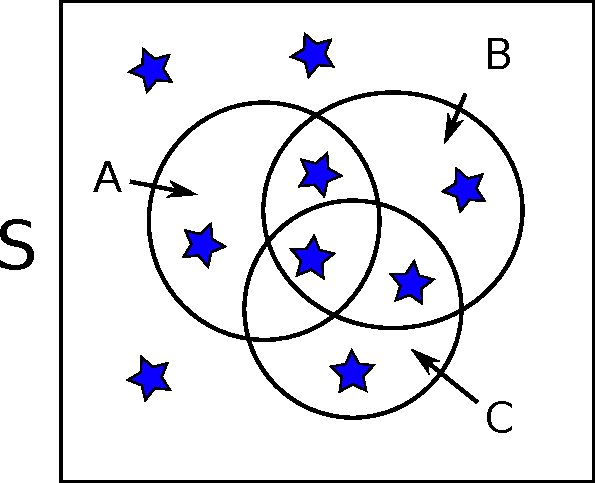
\includegraphics[width=7cm]{inclexcl.pdf}
\end{center}
\begin{enumerate}
\item How many outcomes are there in $S$ in total?
\begin{Freeform}{9}
\# outcomes = 
\Hint Each outcome is represented as a star--just count the number of stars.
\end{Freeform}
%-----------------------------------
\item How many outcomes are in the union $A \cup B \cup C$?
\begin{Freeform}{6}
\# outcomes = 
\Hint Each outcome is represented as a star--just count the number of stars in $A,B$, and $C$.
\end{Freeform}
%-----------------------------------
\item What is $\Prob[A \cup B \cup C]$? Please enter your answer as a fully reduced fraction (i.e. in the form $x/y$ where $x,y$ are the smallest possible integers they can be).
\begin{Freeform}{2/3}
$\Prob[A \cup B \cup C]$ = 
\Hint Review the definition of probability in a discrete space.
\end{Freeform}
%-----------------------------------
\item Now, we will calculate this probability using the Principle of Inclusion-Exclusion. First, what is $ \Prob[A] + \Prob[B] + \Prob[C]$? Please enter your answer as a fully reduced fraction (i.e. in the form $x/y$ where $x,y$ are the smallest possible integers they can be).
\begin{Freeform}{10/9}
$ \Prob[A] + \Prob[B] + \Prob[C]$ = 
\Hint Review the definition of probability in a discrete space--how many outcomes fall in each of the events $A, B, C$? Take a sum of each of the individual probabilities.
\end{Freeform}
%-----------------------------------
\item Notice that the above was a severe overestimate of $\Prob[A \cup B \cup C]$. This is because all of the two-way intersections were counted twice, once for each individual event. 

Now, calculate the sum of probabilities of the intersections, $\Prob[A \cap B] + \Prob[B \cap C] + \Prob[C \cap A]$. Please enter your answer as a fully reduced fraction (i.e. in the form $x/y$ where $x,y$ are the smallest possible integers they can be).
\begin{Freeform}{5/9}
$\Prob[A \cap B] + \Prob[B \cap C] + \Prob[C \cap A]$ = 
\Hint Review the definition of probability in a discrete space--how many outcomes fall in each of the two-way intersections of the events? Take a sum of each of the individual probabilities.
\end{Freeform}
%-----------------------------------
\item Now, subtract the two-way intersections from the sum of the individual probabilities. What is $\Prob[A] + \Prob[B] + \Prob[C] - (\Prob[A \cap B] + \Prob[B \cap C] + \Prob[C \cap A])$?. Please enter your answer as a fully reduced fraction (i.e. in the form $x/y$ where $x,y$ are the smallest possible integers they can be).
\begin{Freeform}{5/9}
$\Prob[A] + \Prob[B] + \Prob[C] - (\Prob[A \cap B] + \Prob[B \cap C] + \Prob[C \cap A])$ = 
\Hint Simply subtract your answer from part (e) from your answer in part (d), and ensure that your input is of the proper form.
\end{Freeform}
%-----------------------------------
\item Finally, notice that this probability is slightly less than $\Prob[A \cup B \cup C]$. This is because the 3-way intersection was originally added 3 times, but then subtracted 3 times, which is once too many. 

What is $\Prob[A \cap B \cap C]$? Please enter your answer as a fully reduced fraction (i.e. in the form $x/y$ where $x,y$ are the smallest possible integers they can be).
\begin{Freeform}{1/9}
$\Prob[A \cap B \cap C]$ = 
\Hint Review the definition of probability in a discrete space--how many outcomes fall in $A \cap B \cap C$?
\end{Freeform}
%-----------------------------------
\item Now, add back $\Prob[A \cap B \cap C]$ to your answer in the part (f). Does this probability match the probability you calculated in part (c)?
\begin{Multi}
\begin{itemize}
\TrueChoice\item Yes
\FalseChoice\item No
\end{itemize}
\end{Multi}
\end{enumerate}

%------------------------------------------------------------------------------------------------------------------------

\item {\bf Balls and Bins.} Suppose you have $m$ labeled balls $a_1, \ldots, a_m$ that you have thrown one by one, uniformly at random into $n$ labeled bins $b_1, \ldots, b_n$. For each of the probabilities below, select all answers that apply from the list of choices.
\begin{enumerate}
\item What is the probability that $b_j$ contains $a_i$? Select all answers that apply.
\begin{Choices}
When $a_i$ is being thrown, what is the probability that it lands in $b_j$? How many choices are there?
\begin{enumerate}
\FalseChoice\item $\left(1 -\frac{1}{n}\right)^m$
\TrueChoice\item $\frac{1}{n}$
\FalseChoice\item $\frac{1}{m}$
\FalseChoice\item $\frac{m}{n}$
\end{enumerate}
\end{Choices}
%-----------------------------------
\item What is the probability that $b_j$ is empty? Select all answers that apply.
\begin{Choices}
For each ball, what is the probability that it does not end up in $b_j$? Are these events independent?
\begin{enumerate}
\TrueChoice\item $\left(1 -\frac{1}{n}\right)^m$
\TrueChoice\item $\binom{m}{0}\cdot\left(1 -\frac{1}{n}\right)^m$
\FalseChoice\item $\frac{1}{m!}$
\FalseChoice\item $\frac{1}{n!}$
\end{enumerate}
\end{Choices}
%-----------------------------------
\item What is the probability that $b_j$ contains all of the balls? Select all answers that apply.
\begin{Choices}
For each ball, what is the probability that it ends up in $b_j$? Are these events independent?
\begin{enumerate}
\FalseChoice\item $\left(1-\frac{1}{n}\right)^m$
\TrueChoice\item $\left(\frac{1}{n}\right)^m$
\TrueChoice\item $\binom{m}{m}\cdot\left(\frac{1}{n}\right)^m$
\FalseChoice\item $\frac{1}{m!}$
\end{enumerate}
\end{Choices}
%-----------------------------------
\item What is the probability that $b_j$ contains exactly $k$ balls? Select all answers that apply.
\begin{Choices}
For each ball, what is the probability that it ends up in $b_j$? Are these events independent? Does order matter?
\begin{enumerate}
\FalseChoice\item $\binom{m}{k}\cdot\left(\frac{1}{n}\right)^{m-k}\cdot \left(1-\frac{1}{n}\right)^{k}$
\FalseChoice\item $\left(\frac{1}{n}\right)^{k}\cdot \left(1-\frac{1}{n}\right)^{m-k}$
\TrueChoice\item $\binom{m}{k}\cdot\left(\frac{1}{n}\right)^{k}\cdot \left(1-\frac{1}{n}\right)^{m-k}$
\FalseChoice\item $\left(\frac{1}{n}\right)^{k}$
\end{enumerate}
\end{Choices}
%-----------------------------------
\item What is the probability that $b_j$ contains at most $k$ balls?
\begin{Choices}
What is the probability that $b_j$ contains exactly $i$ balls? Review the probability of a union of disjoint events in note 10.
\begin{enumerate}
\FalseChoice\item $\sum_{i = 0}^{k}\binom{m}{i}\cdot\left(\frac{1}{n}\right)^{m-i}\cdot \left(1-\frac{1}{n}\right)^{i}$
\TrueChoice\item $\sum_{i = 0}^{k} \binom{m}{i}\cdot\left(\frac{1}{n}\right)^{i}\cdot \left(1-\frac{1}{n}\right)^{m-i}$
\TrueChoice\item $1 - \sum_{i = k+1}^{m}\binom{m}{i}\cdot\left(\frac{1}{n}\right)^{i}\cdot \left(1-\frac{1}{n}\right)^{m-i}$
\TrueChoice\item $1 - \sum_{i = 0}^{m-k}\binom{m}{i}\cdot\left(\frac{1}{n}\right)^{m-i}\cdot \left(1-\frac{1}{n}\right)^{i}$
\end{enumerate}
\end{Choices}
\end{enumerate}
%-----------------------------------
\item {\bf Processes, servers and overloading.} I have $M$ processes (jobs) and 
    $N$ servers that I can assign the jobs to. Any job may be assigned to any 
    server. Suppose I assign each job to a randomly chosen server, with all 
    servers being equally likely. We say that a server is overloaded if it is 
    assigned greater than or equal to $K$ jobs, where $K \leq M$. What is the 
    probability that the first server is overloaded?
\begin{Choices}
\begin{enumerate}
    \FalseChoice\item $\sum_{i=0}^{M-K-1} \dbinom{M}{K+i} \frac{(N-1)^{M-K-i}}{N^{M}}$
    \FalseChoice\item $\sum_{i=0}^{N-K} \dbinom{N}{K+i} \frac{(M-1)^{N-K-i}}{M^{N}}$
    \TrueChoice\item $\sum_{i=0}^{M-K} \dbinom{M}{K+i} \frac{(N-1)^{M-K-i}}{N^{M}}$
    \FalseChoice\item $\dbinom{M}{K} \frac{(N-1)^{M-K}}{N^{M}}$
    \FalseChoice\item $\left(\frac{N-1}{N}\right)^{M-K}$
\end{enumerate}
\end{Choices}
%-----------------------------------
\item {\bf Jobs and servers, without immediate repetition.} I have $M\geq 2$ 
    jobs and $N \geq M$ servers to assign the jobs to.
    
    I use the following system to assign the jobs: the 
    first job is randomly assigned to one of the $N$ servers (with all servers 
    being equally likely). The second job is again assigned randomly to a 
    server, except that the server that got the first job is excluded from the 
    selection (any of the other $N-1$ servers are equally likely to get the job). 
    Similarly, the third job is assigned randomly, except this time, the 
    server that got the second job is excluded (any of the other $N-1$ servers 
    have equal likelihood of being chosen for this job). And so on until all 
    $M$ jobs have been assigned.

    What is the probability that each of the $M$ jobs goes to a different 
    server?
\begin{Choices}
\begin{enumerate}
    \FalseChoice\item $\sum_{i=0}^{N-M}\frac{(N-i-2)!}{(N-M-i)! (N-1)^{M-2}}$
    \FalseChoice\item $\frac{(M-2)!}{(N-M)! (M-2)^{N-1}}$
    \FalseChoice\item $\frac{(N-1)!}{(N-M)! N^{M-1}}$
    \FalseChoice\item $\frac{(N-2)!}{(N-M)! (N-2)^{M-3}}$
    \TrueChoice\item $\frac{(N-2)!}{(N-M)! (N-1)^{M-2}}$
\end{enumerate}
\end{Choices}
%-----------------------------------
\item {\bf Bounding overload probabilities.} I have a load balancing set up 
    with $N$ servers, where I can guarantee that the probability of the $i^{th}$ 
    server being overloaded (where $1\leq i \leq N$) is at most $p$, which is 
    independent of $i$. Which of the following is true? Check all that apply.
    
   \begin{Multi}
\begin{enumerate}
    \FalseChoice\item $\textnormal{Pr (no server is overloaded)} \leq 1-Np$
    \TrueChoice\item $\textnormal{Pr (no server is overloaded)} \geq 1-Np$
    \TrueChoice\item $\textnormal{Pr (at least one server is overloaded)} \geq p$
    \FalseChoice\item $\textnormal{Pr (no server is overloaded)} \leq 1-N(1-p)$
    \FalseChoice\item $\textnormal{Pr (no server is overloaded)} \geq 1-(1-p)^{2N}$
    \TrueChoice\item $\textnormal{Pr (at least one server is overloaded)} \leq Np$
\end{enumerate}
\end{Multi}

\end{enumerate}
\end{document}
